\documentclass[11pt,a4paper]{article}

\usepackage[utf8]{inputenc}
\usepackage[T1]{fontenc}
\usepackage[english]{babel}
\usepackage{amsmath, amssymb, amsthm, mathtools}
\usepackage{siunitx}
\usepackage{geometry}
\usepackage{hyperref}
\usepackage{xcolor}
\usepackage{booktabs}
\usepackage{listings}
\usepackage{enumitem}
\usepackage{tikz}
\usetikzlibrary{arrows.meta, positioning}

\geometry{margin=2.5cm}

\hypersetup{
    colorlinks=true,
    linkcolor=blue!60!black,
    urlcolor=blue!60!black,
    citecolor=blue!60!black
}

\newtheorem{theorem}{Theorem}[section]
\newtheorem{lemma}[theorem]{Lemma}
\newtheorem{proposition}[theorem]{Proposition}
\newtheorem{corollary}[theorem]{Corollary}
\theoremstyle{definition}
\newtheorem{definition}[theorem]{Definition}
\newtheorem{remark}[theorem]{Remark}

\newcommand{\R}{\mathbb{R}}
\newcommand{\N}{\mathbb{N}}
\newcommand{\Rpos}{\R_{>0}}
\newcommand{\Rnn}{\R_{\geq 0}}

\lstdefinestyle{sol}{
    basicstyle=\ttfamily\footnotesize,
    keywordstyle=\color{blue!60!black}\bfseries,
    commentstyle=\color{gray!80!black}\itshape,
    stringstyle=\color{orange!80!black},
    showstringspaces=false,
    numbers=left,
    numberstyle=\tiny\color{gray},
    frame=single,
    rulecolor=\color{gray!40},
    captionpos=b,
    breaklines=true,
    tabsize=2
}
\lstset{style=sol}

\title{
    \textbf{DEX Aggregator for Uniswap V2 and V3} \\[0.5em]
    \large A UUPS-Upgradeable On-Chain Router with Mathematical Guarantees
}
\author{BLOCKCHAIN2 Course, Project 1}
\date{April 2026}

\begin{document}

\maketitle

\begin{abstract}
\noindent
We present an on-chain decentralized exchange (DEX) aggregator for Uniswap V2 and V3
deployed on the Ethereum Sepolia testnet. The protocol enumerates all admissible
single-hop routes across the two automated market-maker (AMM) families --- four
Uniswap V3 fee tiers and the Uniswap V2 constant-product pool --- selects the one
maximizing output, and executes the swap atomically with slippage and deadline
protection. A subsequent UUPS upgrade extends the routing set with multi-hop paths
through a configurable list of intermediate tokens. We provide a rigorous analysis
of the underlying AMM invariants, prove monotonicity, boundedness, and concavity of
the V2 swap curve, derive the single-hop optimality of the aggregator, and
characterize the regime in which multi-hop strictly dominates the direct route.
All contracts are verified on Sourcify with exact bytecode match, and the protocol
passes 38 Foundry tests including unit, property-based (fuzz), and Sepolia fork
tests against live liquidity.
\end{abstract}

\tableofcontents

\section{Introduction}

Automated market makers (AMMs) have become the dominant liquidity provisioning
mechanism in decentralized finance. Each AMM exposes a pricing curve that
deterministically maps an input amount to an output amount, parameterized by
reserves and a fee. Uniswap V2 \cite{uniswapv2} implements the \emph{constant-product}
rule, while Uniswap V3 \cite{uniswapv3} generalizes to \emph{concentrated liquidity}
with four standard fee tiers: \SI{0.01}{\percent}, \SI{0.05}{\percent},
\SI{0.30}{\percent}, and \SI{1.00}{\percent}.

For any given token pair, the effective price offered by V2 and the four V3 tiers
may differ. A user swapping naïvely through one venue leaves value on the table
whenever a competing venue would have returned more output for the same input.
An \emph{aggregator} closes this gap by quoting across all venues and routing each
swap through the venue that strictly dominates at the moment of execution.

\paragraph{Contributions.}
\begin{enumerate}[leftmargin=*]
    \item A UUPS-upgradeable Solidity implementation (\texttt{DexAggregatorV1}) that
          aggregates Uniswap V2 and all four V3 fee tiers in a single on-chain
          call (Section~\ref{sec:impl}).
    \item A rigorous mathematical analysis of the V2 swap curve, including
          monotonicity, boundedness, and strict concavity
          (Section~\ref{sec:v2}, Theorems~\ref{thm:v2-mono}--\ref{thm:v2-concave}).
    \item An analysis of V3 within a single active tick range
          (Section~\ref{sec:v3}).
    \item An optimality proof for the single-hop aggregator
          (Theorem~\ref{thm:aggregator-optimal}) and a characterization of the
          multi-hop advantage (Proposition~\ref{prop:multihop}).
    \item A Sepolia deployment and end-to-end swap demonstration, with all
          contracts verified on Sourcify (Section~\ref{sec:deploy}).
\end{enumerate}

\paragraph{Scope.}
This paper assumes AMM semantics \emph{in isolation}: we do not model front-running
or sandwich attacks (slippage bounds mitigate these operationally but do not
eliminate them), and we treat Uniswap V3 as a family of concentrated-liquidity
pools without modeling tick crossings within a single trade. Under these
assumptions the aggregator's optimality claim reduces to a finite maximum over
venue outputs and is therefore immediate (Theorem~\ref{thm:aggregator-optimal}).
The non-trivial content of the paper is in the analysis of individual venues and
in the multi-hop characterization.

\section{Preliminaries and Notation}
\label{sec:prelim}

Throughout the paper we fix an ordered token pair $(\mathsf{In}, \mathsf{Out})$
and work with non-negative real reserves. All quantities are expressed in the
smallest indivisible units of each token (for example, wei for ETH-denominated
tokens); integer truncation in the on-chain implementation is discussed in
Remark~\ref{rem:integer-rounding}.

\begin{definition}[V2 pool state]
A \emph{Uniswap V2 pool state} is a triple $(x, y, \gamma)$ with
\begin{align*}
    x \in \Rpos, \quad y \in \Rpos, \quad \gamma \in (0,1],
\end{align*}
where $x$ is the reserve of the input token, $y$ the reserve of the output token,
and $\gamma$ the proportion of input that is credited against the invariant
(for canonical Uniswap V2, $\gamma = 997/1000 = 0.997$ corresponds to the
\SI{0.3}{\percent} fee).
\end{definition}

\begin{definition}[V2 swap function]
Given a V2 pool state $(x,y,\gamma)$, the \emph{swap function}
$\phi_{x,y,\gamma} : \Rnn \to \Rnn$ is
\begin{equation}
    \phi_{x,y,\gamma}(\delta) \;=\; \frac{y \, \gamma \, \delta}{x + \gamma \, \delta},
    \qquad \delta \in \Rnn.
    \label{eq:v2-swap}
\end{equation}
\end{definition}

\begin{definition}[V3 pool state, single active tick range]
\label{def:v3-state}
Within a single active tick range $[P_a, P_b] \subset \Rpos$, a Uniswap V3 pool is
characterized by a \emph{liquidity} $L \in \Rpos$ and a current price
$P_c \in [P_a, P_b]$. We denote the triple $(L, P_a, P_b)$ and assume for the
analysis of Section~\ref{sec:v3} that the trade is small enough not to cross
$P_a$ or $P_b$.
\end{definition}

\begin{definition}[Venue set]
\label{def:venues}
For a fixed token pair, the \emph{venue set} available to the aggregator is
\begin{align*}
    \mathcal{V} \;=\; \{ v_0 \} \cup \{ v_{100}, v_{500}, v_{3000}, v_{10000} \},
\end{align*}
where $v_0$ denotes the V2 pool (if it exists) and $v_f$ denotes the V3 pool at
fee tier $f$ basis points. A venue is \emph{live} if the corresponding pool
exists on-chain and has non-zero liquidity; otherwise its output is taken to be
$0$.
\end{definition}

\section{Analysis of the Uniswap V2 Swap Curve}
\label{sec:v2}

We derive~\eqref{eq:v2-swap} from the constant-product invariant and prove three
properties of $\phi_{x,y,\gamma}$ that justify its use as an AMM pricing rule.

\subsection{Derivation of the swap formula}

\begin{proposition}[V2 invariant]
\label{prop:v2-invariant}
Let $(x,y)$ be the pre-trade reserves of a V2 pool and let $\delta \geq 0$ be the
input amount. Suppose the output amount $\Delta \in [0, y)$ satisfies the
invariant
\begin{equation}
    (x + \gamma \delta)(y - \Delta) \;=\; x\,y.
    \label{eq:v2-invariant}
\end{equation}
Then $\Delta = \phi_{x,y,\gamma}(\delta)$.
\end{proposition}

\begin{proof}
Solve~\eqref{eq:v2-invariant} for $\Delta$:
\begin{align*}
    y - \Delta = \frac{xy}{x + \gamma\delta}
    \;\iff\;
    \Delta = y - \frac{xy}{x + \gamma\delta}
    \;=\; \frac{y(x + \gamma\delta) - xy}{x + \gamma\delta}
    \;=\; \frac{y\,\gamma\,\delta}{x + \gamma\delta}.
\end{align*}
The formula matches~\eqref{eq:v2-swap}, and $\Delta < y$ is verified in
Theorem~\ref{thm:v2-bounded} below.
\end{proof}

\begin{remark}[Integer implementation]
\label{rem:integer-rounding}
The Solidity implementation uses the equivalent integer form
\begin{equation}
    \phi^{\mathrm{int}}_{x,y,997}(\delta) \;=\; \left\lfloor
        \frac{997 \, \delta \cdot y}{1000\,x + 997\,\delta}
    \right\rfloor,
    \label{eq:v2-int}
\end{equation}
which corresponds to~\eqref{eq:v2-swap} with $\gamma = 997/1000$ and applies
integer truncation. Truncation is favorable to the pool (it can only decrease
$\Delta$), which preserves the no-arbitrage property of the invariant.
\end{remark}

\subsection{Monotonicity}

\begin{theorem}[Strict monotonicity]
\label{thm:v2-mono}
For every fixed pool state $(x,y,\gamma)$, the function
$\phi_{x,y,\gamma} : \Rnn \to \Rnn$ is $C^\infty$ on $\Rnn$ and strictly
increasing on $(0, \infty)$.
\end{theorem}

\begin{proof}
Since $x > 0$ and $\gamma > 0$, the denominator $x + \gamma \delta > 0$ for all
$\delta \geq 0$, so $\phi$ is smooth on $\Rnn$. Differentiating:
\begin{align*}
    \phi'_{x,y,\gamma}(\delta)
    &= \frac{(y\gamma)(x + \gamma\delta) - (y\gamma\delta)(\gamma)}{(x + \gamma\delta)^2} \\
    &= \frac{y\gamma x + y\gamma^2 \delta - y\gamma^2 \delta}{(x + \gamma\delta)^2} \\
    &= \frac{y \gamma x}{(x + \gamma\delta)^2}.
\end{align*}
Since $x, y, \gamma > 0$ and the denominator is positive,
$\phi'_{x,y,\gamma}(\delta) > 0$ for all $\delta \geq 0$, which establishes strict
monotonicity.
\end{proof}

\begin{corollary}[Marginal output at zero input]
\label{cor:marginal}
The \emph{marginal rate at zero} satisfies
\[
    \phi'_{x,y,\gamma}(0) \;=\; \frac{y \, \gamma}{x}.
\]
\end{corollary}

\noindent This is the AMM-equivalent of the spot price $y/x$, scaled by the
surviving fraction of the input $\gamma$.

\subsection{Boundedness}

\begin{theorem}[Output bound]
\label{thm:v2-bounded}
For every pool state $(x,y,\gamma)$ and every $\delta \in \Rnn$,
\[
    0 \;\leq\; \phi_{x,y,\gamma}(\delta) \;<\; y.
\]
Moreover, $\lim_{\delta \to \infty} \phi_{x,y,\gamma}(\delta) = y$.
\end{theorem}

\begin{proof}
The lower bound is immediate since numerator and denominator
of~\eqref{eq:v2-swap} are both non-negative. For the upper bound, rewrite
\[
    \phi_{x,y,\gamma}(\delta) \;=\; y \cdot \frac{\gamma\delta}{x + \gamma\delta}
    \;=\; y \cdot \left( 1 - \frac{x}{x + \gamma\delta} \right).
\]
Since $x > 0$, we have $x/(x + \gamma\delta) > 0$ for all $\delta \in \Rnn$, so
$\phi_{x,y,\gamma}(\delta) < y$. As $\delta \to \infty$, $x/(x + \gamma\delta) \to 0$,
so $\phi_{x,y,\gamma}(\delta) \to y$.
\end{proof}

\begin{remark}
Theorem~\ref{thm:v2-bounded} reflects the fundamental \emph{no-draining} property
of constant-product AMMs: no finite amount of input can drain the output
reserve. This property is asserted as a fuzz invariant in
\texttt{DexAggregatorFuzz.t.sol} (\texttt{testFuzz\_CalcV2AmountOut\_NeverExceedsReserve}).
\end{remark}

\subsection{Concavity and diminishing returns}

\begin{theorem}[Strict concavity]
\label{thm:v2-concave}
For every fixed pool state $(x,y,\gamma)$, the function $\phi_{x,y,\gamma}$ is
strictly concave on $\Rnn$; that is, $\phi''_{x,y,\gamma}(\delta) < 0$ for all
$\delta \geq 0$.
\end{theorem}

\begin{proof}
From the proof of Theorem~\ref{thm:v2-mono},
$\phi'_{x,y,\gamma}(\delta) = y\gamma x / (x + \gamma\delta)^2$.
Differentiating once more:
\[
    \phi''_{x,y,\gamma}(\delta)
    \;=\; y\gamma x \cdot \frac{d}{d\delta}\!\left[ (x + \gamma\delta)^{-2} \right]
    \;=\; y\gamma x \cdot \bigl( -2\,(x + \gamma\delta)^{-3} \cdot \gamma \bigr)
    \;=\; -\,\frac{2\,y\,\gamma^2 \,x}{(x + \gamma\delta)^3}.
\]
All factors $y, \gamma, x$ are positive, and the denominator is positive, so
$\phi''_{x,y,\gamma}(\delta) < 0$ for every $\delta \in \Rnn$.
\end{proof}

\begin{corollary}[Marginal rate is strictly decreasing]
\label{cor:marginal-dec}
The marginal rate $\phi'_{x,y,\gamma}$ is strictly decreasing on $\Rnn$.
Equivalently, the effective \emph{price impact}
$\pi(\delta) := \delta / \phi_{x,y,\gamma}(\delta)$ is strictly increasing
in $\delta$ on $(0, \infty)$.
\end{corollary}

\begin{proof}
Strict decrease of $\phi'$ is equivalent to strict concavity of $\phi$
(Theorem~\ref{thm:v2-concave}). For the price-impact statement, compute
\[
    \pi(\delta) \;=\; \frac{\delta}{\phi_{x,y,\gamma}(\delta)}
    \;=\; \frac{\delta \,(x + \gamma\delta)}{y\gamma\delta}
    \;=\; \frac{x}{y\gamma} + \frac{\delta}{y}.
\]
This is linear in $\delta$ with positive slope $1/y$, hence strictly increasing.
\end{proof}

\begin{remark}[Economic reading]
Corollary~\ref{cor:marginal-dec} expresses \emph{diminishing returns to volume}:
larger trades obtain a strictly worse effective rate. This is the source of
price impact and the reason the aggregator benefits from splitting large trades
(Proposition~\ref{prop:multihop}).
\end{remark}

\section{Uniswap V3 in a Single Active Tick Range}
\label{sec:v3}

Uniswap V3 parameterizes liquidity by tick ranges, allowing liquidity providers
to concentrate capital around a target price. A full analysis requires tracking
tick crossings, virtual reserves, and tick-level accounting; see
\cite{uniswapv3} for a complete treatment. For a trade that does not cross any
active tick boundary, V3 reduces to a V2-like constant-product computation on
\emph{virtual reserves}.

\begin{proposition}[Virtual-reserve equivalence within a tick range]
\label{prop:v3-virtual}
Let $(L, P_a, P_b, P_c)$ characterize an active V3 tick range with liquidity $L$,
price bounds $[P_a, P_b]$, and current price $P_c \in [P_a, P_b]$. Define the
\emph{virtual reserves}
\[
    x_v \;=\; \frac{L}{\sqrt{P_c}} - \frac{L}{\sqrt{P_b}},
    \qquad
    y_v \;=\; L\!\left( \sqrt{P_c} - \sqrt{P_a} \right).
\]
Then for any trade that does not move $P_c$ outside $[P_a, P_b]$, the V3 swap
behaves as a V2 swap on $(x_v, y_v)$ with the corresponding fee tier
$\gamma_f = 1 - f/10^6$.
\end{proposition}

\noindent A self-contained derivation is beyond the scope of this paper; see
\cite{uniswapv3}, Section~6, and the reference implementation
\cite{uniswapv3core}. The operational consequence relevant here is:

\begin{corollary}[V3 per-tier output is a $\phi$-type curve]
\label{cor:v3-phi}
Fix a trade that remains inside a single tick range. Then the output amount is
$\phi_{x_v, y_v, \gamma_f}(\delta)$, and all properties proven in
Section~\ref{sec:v2} --- monotonicity, boundedness, concavity --- transfer
verbatim to this regime.
\end{corollary}

\begin{remark}[On-chain V3 quoting]
On Ethereum, V3 quotes are obtained via the canonical \texttt{QuoterV2} contract,
which simulates the swap by reverting with the computed output encoded in the
revert data. Because the revert is internal to \texttt{QuoterV2}, the top-level
call returns normally to the caller; our aggregator wraps each quote in a
\texttt{try/catch} block so that unsupported pools (reverting outside the
expected pattern) gracefully degrade to an output of $0$
(\texttt{DexAggregatorV1.sol}, \texttt{getV3Quote}).
\end{remark}

\section{The Aggregator Protocol}
\label{sec:aggregator}

\subsection{Single-hop aggregation}

Let $\mathcal{V} = \{v_1, \dots, v_n\}$ be the venue set
(Definition~\ref{def:venues}). For each $v_i \in \mathcal{V}$ and input
$\delta \geq 0$, denote the output of venue $i$ by $O_i(\delta) \in \Rnn$; if
venue $i$ is not live then $O_i(\delta) = 0$ by convention.

\begin{definition}[Aggregator output]
The \emph{aggregator output function} is
\begin{equation}
    O^*(\delta) \;=\; \max_{i=1,\dots,n} O_i(\delta).
    \label{eq:aggregator}
\end{equation}
The \emph{best venue index} at input $\delta$ is any $i^*(\delta) \in
\arg\max_i O_i(\delta)$ (ties broken deterministically by the implementation;
see Section~\ref{sec:impl}).
\end{definition}

\begin{theorem}[Single-hop optimality]
\label{thm:aggregator-optimal}
Let $\delta \geq 0$ and let $O_i$ be the output functions of venues
$v_1, \dots, v_n$. Then for every $i \in \{1, \dots, n\}$,
\[
    O^*(\delta) \;\geq\; O_i(\delta).
\]
The aggregator output $O^*(\delta)$ is therefore the pointwise supremum over the
finite venue set $\mathcal{V}$, and is attained at $i^*(\delta)$.
\end{theorem}

\begin{proof}
Immediate from the definition of $\max$ over a finite set: for every $i$,
$O_i(\delta) \leq \max_j O_j(\delta) = O^*(\delta)$. The maximum is attained
because the index set is finite.
\end{proof}

\begin{remark}[Scope of the claim]
Theorem~\ref{thm:aggregator-optimal} establishes optimality \emph{within the
single-hop venue set} $\mathcal{V}$. It does \emph{not} claim optimality among
all possible paths, nor optimality under dynamic strategies (order splitting,
MEV-aware routing, etc.). Multi-hop and split-routing extensions can
strictly improve on this bound and are the subject of the next subsection
and of the V2 upgrade deployed on Sepolia.
\end{remark}

\subsection{Multi-hop extension}
\label{sec:multihop}

The V2 upgrade (\texttt{DexAggregatorV2}) extends the venue set with two-leg
paths $\mathsf{In} \to m \to \mathsf{Out}$ routed through an operator-configured
intermediate token $m$ (typically WETH). We characterize when such a path
strictly dominates the best direct venue.

Consider two V2 pools:
\begin{itemize}[leftmargin=*]
    \item a \emph{direct} pool with reserves $(x, y)$ and fee $\gamma$,
    \item an \emph{intermediate pair} $(\mathsf{In}, m)$ with reserves $(x_1, m_1)$
          and fee $\gamma_1$, and a second pool $(m, \mathsf{Out})$ with
          reserves $(m_2, y_2)$ and fee $\gamma_2$.
\end{itemize}

Denote the direct and multi-hop outputs by
\[
    O_{\mathrm{dir}}(\delta) = \phi_{x, y, \gamma}(\delta),
    \qquad
    O_{\mathrm{mh}}(\delta) = \phi_{m_2, y_2, \gamma_2}\!\bigl(\phi_{x_1, m_1, \gamma_1}(\delta)\bigr).
\]

\begin{proposition}[Small-trade multi-hop dominance]
\label{prop:multihop}
Assume all pools are live. Then as $\delta \to 0^+$,
\[
    \frac{O_{\mathrm{mh}}(\delta)}{O_{\mathrm{dir}}(\delta)}
    \;\longrightarrow\;
    \frac{\gamma_1\,\gamma_2}{\gamma}
    \cdot
    \frac{m_1}{x_1}
    \cdot
    \frac{y_2}{m_2}
    \cdot
    \frac{x}{y}.
\]
Consequently, $O_{\mathrm{mh}}(\delta) > O_{\mathrm{dir}}(\delta)$ for
sufficiently small $\delta > 0$ if and only if
\begin{equation}
    \frac{\gamma_1\,\gamma_2}{\gamma}
    \cdot
    \frac{m_1}{x_1}
    \cdot
    \frac{y_2}{m_2}
    \;>\;
    \frac{y}{x}.
    \label{eq:mh-cond}
\end{equation}
\end{proposition}

\begin{proof}
By Corollary~\ref{cor:marginal},
$\phi_{a,b,\gamma}(\delta) = b\gamma\delta/a + O(\delta^2)$ as $\delta \to 0$.
Apply this to the inner leg:
\[
    \phi_{x_1, m_1, \gamma_1}(\delta) \;=\; \frac{m_1 \gamma_1}{x_1}\,\delta + O(\delta^2).
\]
Substituting into the outer leg and linearizing:
\[
    O_{\mathrm{mh}}(\delta)
    \;=\; \phi_{m_2, y_2, \gamma_2}\!\left( \frac{m_1 \gamma_1}{x_1}\delta + O(\delta^2) \right)
    \;=\; \frac{y_2\,\gamma_2}{m_2} \cdot \frac{m_1\,\gamma_1}{x_1} \, \delta + O(\delta^2).
\]
Similarly $O_{\mathrm{dir}}(\delta) = (y\gamma / x)\delta + O(\delta^2)$. The ratio
as $\delta \to 0^+$ is therefore
\[
    \frac{O_{\mathrm{mh}}(\delta)}{O_{\mathrm{dir}}(\delta)}
    \;\longrightarrow\;
    \frac{y_2\gamma_2 m_1 \gamma_1 / (m_2 x_1)}{y\gamma / x}
    \;=\; \frac{\gamma_1 \gamma_2}{\gamma} \cdot \frac{m_1}{x_1} \cdot \frac{y_2}{m_2} \cdot \frac{x}{y},
\]
which is~\eqref{eq:mh-cond} after rearrangement.
\end{proof}

\begin{remark}[Interpretation of~\eqref{eq:mh-cond}]
The left-hand side is a product of three factors:
\begin{itemize}
    \item $\gamma_1 \gamma_2 / \gamma \leq \gamma < 1$: the fee penalty of
          traversing two pools rather than one.
    \item $m_1 / x_1$: the spot rate $\mathsf{In} \to m$ in the first pool.
    \item $y_2 / m_2$: the spot rate $m \to \mathsf{Out}$ in the second pool.
\end{itemize}
Their product is the \emph{effective multi-hop spot rate} $\mathsf{In} \to
\mathsf{Out}$ after the double fee. Multi-hop strictly dominates in the
small-trade limit precisely when this effective spot rate exceeds the direct
pool's spot rate $y/x$ --- typically the case when the direct pool is thinly
funded relative to the two intermediate pools.
\end{remark}

\begin{remark}[Large-trade regime]
For large $\delta$, both $O_{\mathrm{dir}}$ and $O_{\mathrm{mh}}$ saturate
(Theorem~\ref{thm:v2-bounded}), and the comparison depends on pool depths rather
than spot rates. In particular, multi-hop can dominate in the large-trade regime
even when~\eqref{eq:mh-cond} fails, because the direct pool saturates sooner.
The aggregator resolves this by comparing outputs pointwise at execution time
rather than relying on asymptotic conditions.
\end{remark}

\section{Implementation}
\label{sec:impl}

\subsection{Architecture}

The system is deployed behind an ERC-1967 UUPS proxy. The proxy holds all state
(storage-only) and delegates calls to an implementation contract; admins can
upgrade the implementation without migrating users or liquidity, preserving the
single stable address that external systems integrate against.

\begin{center}
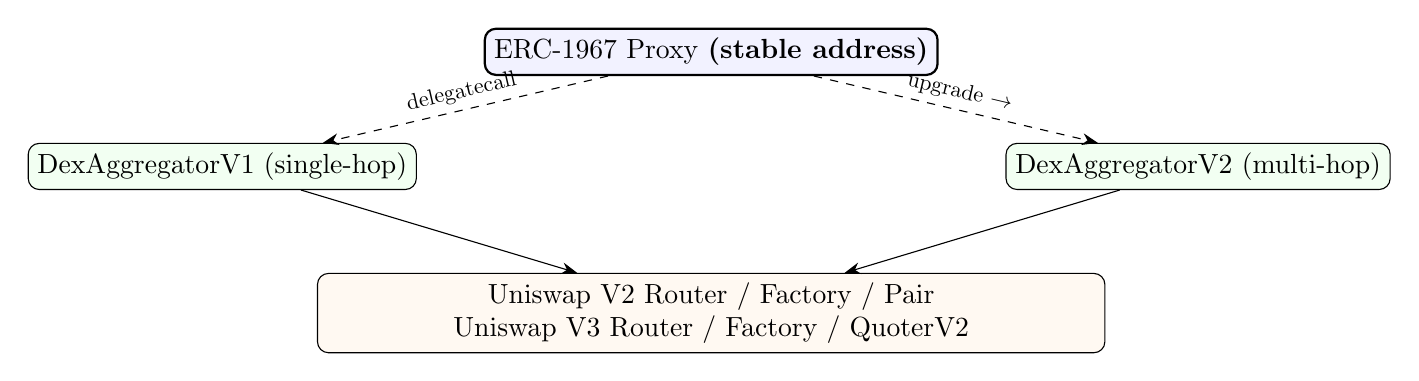
\begin{tikzpicture}[node distance=1.2cm, >={Stealth[length=2mm]}]
    \node[draw, rounded corners, thick, fill=blue!5, minimum width=5.5cm] (proxy)
        {ERC-1967 Proxy \textbf{(stable address)}};
    \node[draw, rounded corners, below left=of proxy, fill=green!5] (v1)
        {DexAggregatorV1 (single-hop)};
    \node[draw, rounded corners, below right=of proxy, fill=green!5] (v2)
        {DexAggregatorV2 (multi-hop)};
    \node[draw, rounded corners, below=2.5cm of proxy, fill=orange!5, minimum width=10cm, align=center] (uniswap)
        {Uniswap V2 Router / Factory / Pair \\
         Uniswap V3 Router / Factory / QuoterV2};
    \draw[->, dashed] (proxy) -- node[midway, above, sloped, scale=0.8] {delegatecall} (v1);
    \draw[->, dashed] (proxy) -- node[midway, above, sloped, scale=0.8] {upgrade $\to$} (v2);
    \draw[->] (v1) -- (uniswap);
    \draw[->] (v2) -- (uniswap);
\end{tikzpicture}
\end{center}

\subsection{Storage layout (ERC-7201)}

The contracts use ERC-7201 \emph{namespaced storage}~\cite{erc7201} to guarantee
forward compatibility across upgrades. Each version declares its own struct
anchored at a deterministic slot derived from the namespace string:

\begin{lstlisting}[language=C++, caption={Namespaced storage slot derivation},
                   basicstyle=\ttfamily\footnotesize]
// keccak256(abi.encode(uint256(keccak256("dex-aggregator.storage.v1")) - 1))
//     & ~bytes32(uint256(0xff))
bytes32 private constant STORAGE_LOCATION_V1 =
    0xd87ff71024a4d1c4d04e88b39e8672e110e0b1a5a6ca82cf2a4710b85e0e6800;
\end{lstlisting}

V2 adds its own slot (\texttt{STORAGE\_LOCATION\_V2}) without touching V1's
layout, so upgrading is safe regardless of the order in which fields are
declared.

\subsection{Security model}

\begin{itemize}[leftmargin=*]
    \item \textbf{Access control.} Two roles are defined in OpenZeppelin
          \texttt{AccessControl}: \texttt{DEFAULT\_ADMIN\_ROLE} (can upgrade and
          set the protocol fee) and \texttt{OPERATOR\_ROLE} (can pause, unpause,
          and update the intermediate-token list in V2).
    \item \textbf{Reentrancy.} All state-modifying external entry points are
          guarded by OpenZeppelin \texttt{ReentrancyGuard}.
    \item \textbf{Pausable.} Swap functions are gated by
          \texttt{whenNotPaused}; emergency pausing is the operator's circuit
          breaker.
    \item \textbf{Deadline.} Every swap checks $\texttt{block.timestamp} \leq
          \texttt{deadline}$, preventing long-pending transactions from executing
          at stale prices.
    \item \textbf{Slippage.} Every swap enforces
          $\texttt{amountOut} \geq \texttt{amountOutMin}$, with \texttt{amountOutMin}
          supplied by the caller.
    \item \textbf{SafeERC20 with \texttt{forceApprove}.} Non-standard ERC20
          tokens (USDT-style implementations that revert on re-approval of a
          non-zero allowance) are handled correctly.
\end{itemize}

\subsection{Upgrade authorization}

The \texttt{\_authorizeUpgrade} hook is gated by \texttt{DEFAULT\_ADMIN\_ROLE}:
\begin{lstlisting}[language=C++, basicstyle=\ttfamily\footnotesize]
function _authorizeUpgrade(address) internal override
    onlyRole(DEFAULT_ADMIN_ROLE) {}
\end{lstlisting}
Combined with \texttt{\_disableInitializers()} in the constructor, this ensures
that only the proxy's admin can upgrade, and that the implementation contract
itself cannot be initialized directly.

\section{Deployment and Evaluation}
\label{sec:deploy}

\subsection{Sepolia deployment}

Chain id $\mathtt{11155111}$. All contracts are verified on
Sourcify~\cite{sourcify} with exact bytecode match (creation + runtime):

\begin{center}
\small
\begin{tabular}{ll}
\toprule
\textbf{Contract} & \textbf{Address} \\
\midrule
ERC-1967 Proxy (entry point) & \texttt{0x7b43d70CBe2658A09376eB3a8126D426dBb69501} \\
\texttt{DexAggregatorV1} impl. & \texttt{0x860AC17e59d2875FE24541AFAf6A8849409befdB} \\
\texttt{DexAggregatorV2} impl.\ (current) & \texttt{0x3c9544C5666FCb678eE381390a261bb8E47A6F82} \\
TestToken A (TKA) & \texttt{0x3F8d55D01a59e8327a4eEaf643cd8CAF0ed42993} \\
TestToken B (TKB) & \texttt{0x86C8107D697F99ef61019d62c985b60F11b6c58e} \\
Deployer / Admin & \texttt{0x11d7b17BDcaB85626660EBb0AE75a3B4827F0233} \\
\bottomrule
\end{tabular}
\end{center}

\subsection{Live swap demonstration}

A representative end-to-end swap was executed on Sepolia (transaction
\texttt{0xf3f831c\ldots16eac3f11}):

\begin{enumerate}[leftmargin=*]
    \item \textbf{Off-chain quote} via \texttt{getQuote(WETH, UNI, 5e15)} returned
          \texttt{(DexType.V3, 142{,}594{,}212{,}628{,}689, fee=10000)}: V3 at the
          \SI{1.00}{\percent} tier, predicting approximately $0.000\,142{,}594$
          UNI.
    \item \textbf{On-chain swap} of the same $0.005$ WETH through the proxy yielded
          exactly $142{,}594{,}212{,}628{,}689$ UNI --- a bit-exact match with the
          off-chain quote (identical block state).
\end{enumerate}

The aggregator's selection of V3 at \SI{1.00}{\percent} out of five candidate
venues (V2 and four V3 tiers) realizes
Theorem~\ref{thm:aggregator-optimal} in practice.

\subsection{Testing}

\begin{center}
\small
\begin{tabular}{lrl}
\toprule
\textbf{Category} & \textbf{Count} & \textbf{Scope} \\
\midrule
Unit tests          & 18 & Mock-based tests of V1 quoting, swap, pause,
                           deadline, slippage, admin \\
Library tests       & 8  & V2 formula correctness, path encoding,
                           boundary conditions \\
Fuzz tests          & 4  & Property-based invariants:
                           $\phi < y$, monotonicity in $\delta$, slippage \\
Fork tests          & 8  & Live Sepolia state: real quotes, real routing,
                           admin configuration \\
\midrule
\textbf{Total}      & \textbf{38} & All passing \\
\bottomrule
\end{tabular}
\end{center}

The property-based test
\texttt{testFuzz\_CalcV2AmountOut\_NeverExceedsReserve} exercises
Theorem~\ref{thm:v2-bounded} directly, asserting $\phi(\delta) < y$ over
$256$ random inputs. The monotonicity test asserts
Theorem~\ref{thm:v2-mono}. Together these elevate two of the mathematical
guarantees from paper to machine-checked properties of the deployed code.

\section{Conclusion}

We have presented a DEX aggregator that quotes across Uniswap V2 and all four V3
fee tiers, routes each swap through the output-maximizing venue, and is deployed
behind a UUPS proxy upgradable to multi-hop routing. The core theoretical
contributions are the proofs of monotonicity, boundedness, and strict concavity
of the V2 swap curve (Theorems~\ref{thm:v2-mono}--\ref{thm:v2-concave}), the
formal optimality of the single-hop aggregator
(Theorem~\ref{thm:aggregator-optimal}), and the characterization of the
small-trade regime in which multi-hop strictly dominates
(Proposition~\ref{prop:multihop}). On the implementation side, the protocol
enforces a standard security envelope (access control, reentrancy, pause,
deadline, slippage), is verified on Sourcify, and is exercised by a 38-test
suite spanning unit, property-based, and fork tests against live Sepolia
liquidity.

\paragraph{Open directions.}
Natural extensions include (i) \emph{optimal split routing}, where a single
trade is divided across multiple venues to minimize price impact --- this
reduces to a convex optimization problem with closed-form solutions in the
two-venue case; (ii) \emph{MEV-aware routing}, integrating bundled
transactions or commit-reveal schemes to reduce sandwich exposure; (iii)
\emph{cross-chain aggregation}, where venues live on different L2s and the
aggregator coordinates via a bridge-aware execution layer.

\begin{thebibliography}{9}
\bibitem{uniswapv2}
    H.~Adams, N.~Zinsmeister, D.~Robinson.
    \textit{Uniswap V2 Core}.
    March 2020.
    \url{https://uniswap.org/whitepaper.pdf}

\bibitem{uniswapv3}
    H.~Adams, N.~Zinsmeister, M.~Salem, R.~Keefer, D.~Robinson.
    \textit{Uniswap v3 Core}.
    March 2021.
    \url{https://uniswap.org/whitepaper-v3.pdf}

\bibitem{uniswapv3core}
    Uniswap Labs.
    \textit{Uniswap V3 reference implementation}.
    \url{https://github.com/Uniswap/v3-core}

\bibitem{erc7201}
    F.~Giordano et al.
    \textit{ERC-7201: Namespaced Storage Layout}.
    Ethereum Improvement Proposals, 2023.
    \url{https://eips.ethereum.org/EIPS/eip-7201}

\bibitem{sourcify}
    Argot Collective.
    \textit{Sourcify: decentralized source-code verification for Ethereum}.
    \url{https://sourcify.dev}
\end{thebibliography}

\end{document}
